\chapter{Creating experiment files}
\label{chap:Creating experiment files}

An \apex experiment file is an XML file. Like any XML file, it
contains a root element (\element{apex}), which contains various
main elements. The general structure of an \apex experiment file
could be as follows:

\begin{lstlisting}
<?xml version='1.0' encoding='UTF-8'?>
<apex>
  <procedure xsi:type="apex:adaptiveProcedureType">
    <parameters> ... </parameters>
    <trials> ... </trials>
  </procedure>

  <corrector xsi:type="apex:isequal"/>
  <screens> ... </screens>
  <datablocks> ... </datablocks>
  <devices> ... </devices>
  <stimuli> ... </stimuli>
</apex>
\end{lstlisting}

The main elements are listed in the next section. Subsequently,
each main element is discussed briefly.

\section{Main Apex elements}

Here we describe the main elements of the experiment, and the
order in which they should occur. Some of them are compulsory,
some are optional, and some contain child elements (nested, see
section~\ref{sec:BasicXML:elements,tags,attributes}). Only the
first child element is given. A complete listing of all the
elements is given in the reference manual.


\begin{itemize}
\item \element{description} \emph{optional} A human readable description of the experiment, for your own reference.

\item \element{procedure} see section~\ref{sec:procedures}

\item \element{corrector} see section~\ref{sec:Corrector}

\item \element{screen} see section~\ref{sec:screen}

\item \element{datablocks} see section~\ref{sec:datablocks}

\item \element{devices} see section~\ref{sec:Devices}

\item \element{filters} \emph{optional} see
section~\ref{sec:Filters}

\item \element{stimuli} see section~\ref{sec:Stimuli}

\item \element{connections} \emph{optional} see
section~\ref{sec:Connections}

\item \element{randomgenerators} \emph{optional} used to set
parameters to random values, for example useful to implement level
roving. An example of level roving is given in
section~\ref{sec:roving}

\item \element{calibration} \emph{optional} see
section~\ref{sec:Calibration}

\item \element{results}\emph{optional} see
section~\ref{sec:Results} and section~\ref{sec:Using XSLT
transforms}


\item \element{interactive}\emph{optional} see
section~\ref{sec:Interactive}

\item \element{general}\emph{optional} see
section~\ref{sec:General}
\end{itemize}

In the next paragraphs these elements will be described in more
detail and their main child elements will be given.

\subsection{Declaration of Main \element{apex} element}

To associate an experiment file with the correct name space and
schema, the following attributes are necessary:


\begin{lstlisting}
<apex:apex xmlns:xsi="http://www.w3.org/2001/XMLSchema-instance"
    xsi:schemaLocation="http://www.kuleuven.be/exporl/Lab/Apex"
    xmlns:apex="http://www.kuleuven.be/exporl/Lab/Apex"
    version="1">
...
</apex:apex>
\end{lstlisting}

For more information on name spaces and schema declarations, we
refer to the XML specifications. For \apex it is sufficient to
copy the text above.

One modification to the above attributes can, however, be useful.
If you use an XML editor with schema support (to allow
autocompletion and showing documentation from the schema), it
needs to know where the \apex schema (\filename {apex-schema.xsd})
is located. This can be indicated by adding an absolute or
relative path to the apex schema to the
\attribute{xsi:schemaLocation} attribute on
line~\ref{xml:schemaloc}. If for example \apex is installed in the
default location (\filename{C:/Program Files/apex3}), the result
would be as follows:

\begin{lstlisting}
<apex:apex xmlns:xsi="http://www.w3.org/2001/XMLSchema-instance"
    xsi:schemaLocation="http://www.kuleuven.be/exporl/Lab/Apex (*@\label{xml:schemaloc}@*)
    file:C:/Program\%20Files/apex3/schemas/apex-schema.xsd"
    xmlns:apex="http://www.kuleuven.be/exporl/Lab/Apex"
    version="1">
...
</apex:apex>
\end{lstlisting}

The \attribute{version} attribute is currently always 1, but this
will change in future versions of \apex.


\index{Main Apex elements}

\subsection{Procedures}

\label{sec:procedures}

Procedure controls the flow of an experiment. It decides on the
next screen to be shown and the next stimulus to be presented.
Generally a procedure will make use of a list of predefined
trials.

e.g.
\begin{lstlisting}
<procedure xsi:type="apex:constantProcedureType">
    <parameters>
        ...
    </parameters>

    <trials>
        <trial id="trial1" >
            ...
        </trial>
        <trial id="trial2" >
            ...
        </trial>
    </trials>
</procedure>
\end{lstlisting}

\index{procedure}

The \attribute{xsi:type} attribute determines the type of
procedure that will be used. There are 5 procedure types
implemented:

\begin{description} \item [adaptiveProcedureType:] the dependent variable (eg: level) of the
stimulus depends on the response of the subject \item
[constantProcedureType:] the dependent variable (eg: level) is
fixed and each trial is presented a specified number of times
\item [trainingProcedureType:] a stimulus is presented AFTER the
user has indicated the trial by pressing a button on the screen.
If no corresponding trial is found, an error message box is shown.
This procedure is designed to be used as a drop-in for the
constant procedure to allow subjects to perform training before
starting the actual experiment

\item [pluginProcedureType:] allows the user to implement a custom
procedure using ECMAScript, see section~\ref{sec:plugins}.

\item [multiProcedureType:] contains several child procedures of any of the other 4 types and
selects between them. This procedure ends when all child
procedures have ended
\end{description}

Every \element{procedure} contains the following elements:

\begin{itemize}
\item \element{parameters} specifies the workings of a procedure,
e.g., specifies the number of presentations per trial. Please read
section~\ref{sec:Parameters} \item \element{trials} specifies each
trial that can be presented. A trial consists of a screen to be
shown, a stimulus to be presented and the correct response. Each
of these can be defined here.
\end{itemize}

The procedure determines whether the experiment is completed.

\subsection{Corrector}
\index{corrector}

Corrector corrects the response and hands the results to the
procedure. The type of corrector to be used is defined using the \attribute{xsi:type} attribute.

e.g.

\begin{lstlisting}
    <corrector xsi:type="apex:isequal"/>
\end{lstlisting}

Two main Correctors exist:
\begin{itemize}\item \xml{isequal}: compares whether the text defined in the \element{answer} element in
\element{trial} and the result from the screen (the subject's response) are exactly the same

\item \xml{alternatives}: this corrector is used together with
\element{choices > 1} in \element{procedure/parameters}. The
reader is referred to the reference manual. The Corrector
determines the correct response.
\end{itemize}

\label{sec:Corrector}

\subsection{Screen}
\label{sec:screen}

\index{screen}

\begin{description} \item A screen is a GUI (Graphical User Interface) that is to be used by the subject to
respond to the stimulus that was presented.
\end{description}

\begin{lstlisting}
<screens>
    <reinforcement>
      ...
    </reinforcement>

    <screen id="screenstar_horse_vase_moon">
      ...
    </screen>
</screens>
\end{lstlisting}

\begin{itemize}
\item \element{reinforcement} indicates whether a progress bar is
shown and whether feedback is given

\item \element{screen} a screen is defined for each stimulus. Each
screen has an ID by which it can be referred to elsewhere in the
experiment file (cf in \element{procedure}/\element{trial} ).

\end{itemize}


\subsection{Datablocks}
\label{sec:datablocks}

\index{datablocks}

A datablock is an abstraction of a basic block of data that can be
processed by \apex and can be sent to a matching device. In the
case of a sound card, the datablock would be an audio signal in
the form of a series of samples that is commonly stored on disk as
a so-called wave file.

\begin{lstlisting}
<datablocks>
    <uri_prefix>...</uri_prefix>
    <datablock id="datablock_star">
      ...
    </datablock>
</datablocks>
\end{lstlisting}

Basically, in element \element{datablock}, a wave file on disk is
assigned an ID, such that it can be referred to elsewhere in the
experiment file.

\begin{itemize}
\item \element{uri_prefix} a prefix can be specified inline or by
specifying the ID of a prefix in the \apex config file and setting
attribute \attribute{source} to \xml{apexconfig}. You can specify
a complete URI or part of it. See section~\ref{sec:prefixes}

\item \element{datablock} for each wave file a datablock is
defined, with an ID.
\end{itemize}

\subsection{Devices}
\label{sec:Devices}

\index{devices}

Device is a system connected to the computer that can be
controlled by \apex. Devices can send signals to a transducer.
Examples are sound cards and interfaces to \ac{cis}s. Device(s)
can have parameters that can be controlled by \apex.

\begin{lstlisting}
<devices>
    <device id="wavdevice" xsi:type="apex:wavDeviceType">
      ...
    </device>
</devices>
\end{lstlisting}


\element {device} all devices defined in the experiment file are
grouped in the element Devices

\begin{itemize}

\item wavDeviceType

\item L34Type
\end{itemize}

\subsection{Filters}
\label{sec:Filters}

\index{filters}

Filters are used to process data before sending it to a device.
E.g.: an amplifier (which is a specific kind of filter) can change
the level of a signal during the experiment. (No filter is needed
when the signals are routed directly to the output device).
Currently implemented filters are

\begin{description}
\item \emph {amplifier} for amplifying or attenuating sound data

\item \emph {PluginFilter}, an interface for implementing custom
filters.

\item a special kind of filter is a generator, such as \emph
{SineGenerator}, \emph {NoiseGenerator}, and \emph
{DataLoopGenerator}. The first two generate sine waves and white
noise, respectively. A \emph{DataLoopGenerator} can set a gain,
can loop a given datablock infinitely, and can jump randomly.
\end {description}

\begin{lstlisting}
<filters>
    <filter xsi:type="apex:dataloop" id="noisegen">
    ..
    </filter>
</filters>
\end{lstlisting}

\element{filter} contains those elements which specify a filter or
a generator


\subsection{Stimuli}
\label{sec:Stimuli}

\index{stimuli} Stimuli are the auditory events presented to the
subject. They can consist of one or more datablocks that are
routed to any number of devices, simultaneously or sequentially.

\begin{lstlisting}
<stimuli>
  <fixed_parameters>
  ...
  </fixed_parameters>

  <stimulus id="stimulus_sentence1">
  ...
  </stimulus>
</stimuli>
\end{lstlisting}}


\begin{itemize}
\item \element{fixed_parameters} see section~\ref{sec:Parameters}

\item \element{stimulus}
\end{itemize}

\subsection{Connections}
\label{sec:Connections}

\index{connections}

Connections are defined to connect Datablocks, Filters and Devices. Any
Datablock can be connected to any Filter or Device and any Filter can be connected to any other Filter
or Device.
\begin{lstlisting}
  <connections>
    <connection>
     ...
    </connection>
  </connections>

\end{lstlisting}

\element {connections} defines how the different filters are
routed to the output device(s)


\subsection{Calibration}
\label{sec:Calibration}

\index{calibration}

Calibration consists of a GUI for calibrating parameters and saving and applying
calibration results. Any stimulus defined in the experiment files can be used as a calibration stimulus.

Typically, calibration is the process of measuring which value of
a digital parameter corresponds to a certain physical magnitude ,
e.g., determining which internal amplification is necessary for a
given wave file to achieve a certain sound pressure level.

\apex provides a GUI to ease calibration (figure~\ref{fig:name1}).
\apex can only calibrate parameters, i.e., it can set a parameter
to a certain value such that the resulting physical magnitude is
the one defined in the experiment file in the
\element{calibration} element.

Because often the same calibration is useful for a set of
experiment files, calibrations are stored under so-called
\emph{calibration profiles}. The calibration profile to be used
must be specified in the \element{calibration} element. For
example if multiple experiment files are used for speech in noise
tests, the calibration profile could be \xml{SpeechInNoise}.

As it is possible to use \apex on the same computer with the same
experiment files in different contexts (e.g., different types of
headphones, which have different calibration settings), \apex
makes use of the concept \emph{hardware setup}. A hardware setup
associates a label to a certain set of hardware devices. The
current hardware setup can be selected at runtime, i.e., cannot be
specified in the experiment file.

If \element{calibration} is defined in the experiment file and the
calibration profile has not been calibrated before for the current
hardware setup, the calibration window will be shown at the start
of the experiment. The first time calibration is used at all, the
window with the hardware setup will appear automatically.


If the calibration profile was calibrated before, but you wish to
recalibrate or change the current hardware setup, select
\emph{Recalibrate} from the menu, select \emph{Manage profiles}
and add the desired label for the current hardware configuration,
eg. ``RME + headphones'', and click \textbf{Add} and \textbf{OK}.
This configuration will also appear in the \apex window in the
lower right hand corner. Under \textbf{Details...} the different
calibration profiles that have been calibrated before will be
shown (figure~\ref{fig:name2}).

On the left hand side of the main calibration window the
parameters to be calibrated are shown (as specified in the
\element{calibration} element in the experiment file). In this
example the parameter \id{cardgain} is calibrated, i.e. the gain
of the sound card. First allow the calibration stimulus ample time
to be able to measure an accurate value with a measuring device or
use the averaging function of the device. Enter the measured
amplitude (in \textbf{Measured amplitude}) and click on
'\textbf{Correct output parameter}'. Repeat until the intended and
measured values are the same. To save the result, click
\textbf{apply}, and click on the OK button.  \apex will store this
profile and retrieve it each time it is used.


Important
\begin{itemize}

\item Remember to check whether the correct \emph{Hardware setup}
is selected when starting an experiment. \apex will always use the
hardware setup used in the previous experiment unless otherwise
specified.

\item \textbf{Apply} and \textbf{OK}. Each calibrated parameter
needs to be saved by clicking on Apply and after all parameters
are calibrated clicking on OK at the bottom of the dialog.
\end{itemize}

It can be of interest to calibrate at a higher level than the
desired stimulation level, to avoid interference of background
noise. If a yellow message appears, the signal has clipped.


The calibration is user dependent. After having logged in it is
possible to import or export the own calibration files.


\begin{figure}
 \centering
%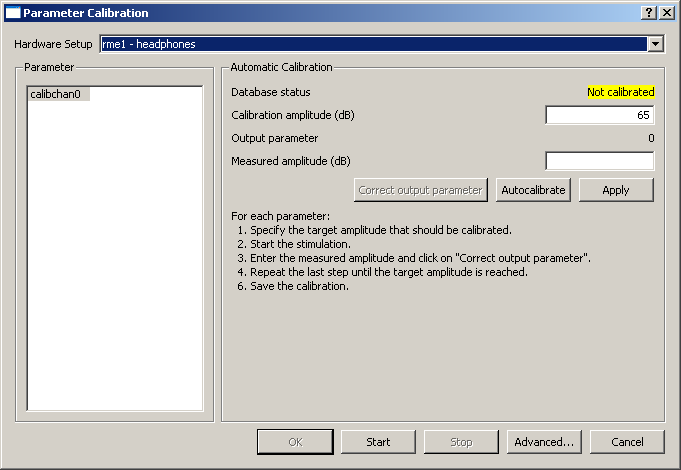
\includegraphics[width=\textwidth]{calibrationwindow.png}
 \caption{The calibration window}
 \label{fig:name1}
\end{figure}


\begin{figure}
 \centering
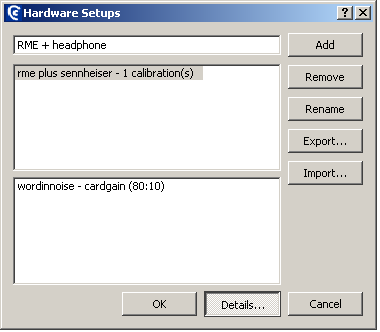
\includegraphics[width=0.5\textwidth]{calibrationwindow2.png}
 \caption{The calibration window showing \emph{Manage profiles}}
 \label{fig:name2}
\end{figure}
\label{sec:Calibration}


 \index{calibration}


\subsection{Results}
\label{sec:Results}


\index{results}

After completion of the experiment a file containing results is
always delivered, even if it is not specified in the experiment
file. The default results file is in XML and it contains all the
information about the course of the completed experiment. Please
read section~\ref{chap:Results}.

\subsection{Interactive}
\index{Interactive}

\label{sec:Interactive}

Interactive allows the experimenter to modify certain aspects of
the experiment file right before the experiment is started using a
GUI.


\begin{itemize}
\item \element{Entry}
\end{itemize}

\subsection{General}
General defines some general parameters.

\label{sec:General}
\begin{itemize}
\item \element{show_results}

\item \element{saveprocessedresults}
\end{itemize}
\index{General}

\section{Parameters}
\index{parameters}

There are two types of parameters:
\begin{description}

\item [fixed parameter:] a fixed parameter is a property of a
stimulus. It cannot be changed by \apex at runtime and is defined
when the experiment file is created. It can be used by the
procedure to select a stimulus from a list, it can be shown on the
screen or it can be used as a piece of information when analyzing
results

\begin{lstlisting}
<stimuli>
    <fixed_parameters>
      <parameter id="gap"/>
    </fixed_parameters>

    <stimulus id="stimulus1" >
    <description>noisewithgap1</description>
      <datablocks>
        <datablock id="gwith5msinterval" />
      </datablocks>
      <fixedParameters>
            <parameter id="gap">5</parameter>
      </fixedParameters>
    </stimulus>
    ....
</stimuli>
\end{lstlisting}

Fixed parameters are often used by adaptive procedures. If a
certain fixed parameter is selected to be adapted by a procedure,
the stimulus to be presented will be selected using that fixed
parameter. The stimuli are selected amongst those listed in the
current trial. In this example the duration of the gap is varied
in a gap detection task.

 \item [variable parameter:] a variable parameter is a
property of an object of which the value can be changed at
runtime. Variable parameters can be set by various \apex modules.
Examples of modules that can define variable parameters are
AdaptiveProcedure, Calibrator and Screen. Variable parameters can
also be defined by Stimulus. If a stimulus description contains a
variable parameter, it will be set just before the stimulus is
presented. Examples of modules that can have variable parameters
(to be set by another module) are Filter, Controller and Device.
\end{description}.

\begin{lstlisting}

 <stimuli>
  <fixed_parameters/>
   <stimulus id="stimulus0">
      <description>Stimulus0</description>
      <datablocks>
        <datablock id="datablock0"/>
      </datablocks>
      <variableParameters>
        <parameter id="speaker">3</parameter>
        </variableParameters>
        <fixedParameters/>
    </stimulus>
</stimuli>

\end{lstlisting}


\label{sec:Parameters}

A variable stimulus parameter, is a parameter that will be set
elsewhere just before the stimulus is sent to the device. A
variable parameter should be defined elsewhere (eg. in a filter,
in a device, ..).

e.g. In examples 1 and 2 the gain of an amplifier is made a
variable parameter by assigning it ID \id{gain}


\subsection{Apexconfig}
\label{apexconfig}


The \filename{apexconfig.xml} file is a configuration file that
applies to all experiments. It is stored in the folder
\filename{config}, under the main \apex folder. It includes common
names of sound cards and drivers and prefixes that can be referred
to from any experiment file.

If the \filename{apexconfig.xml} is not defined for a current user
a generic file will be used. It is, however, also possible to have
an \filename{apexconfig.xml} file per user. To add an
\filename{apexconfig.xml} file for a specific user, log in as the
user, and copy the apexconfig.xml file to the folder
\filename{C:/Documents and Settings/your Windows Login
name/Application Data/ExpORL}. If the file
\filename{apexconfig.xml} is present in the latter folder, it will
override the \filename{apexconfig.xml} file in the config folder
under main \apex directory.

\index{apexconfig}

\section{Using prefixes}

When specifying a prefix in an experiment file (e.g. in
\element{datablocks} or \element{screens}), it is possible, but
not necessary to write out the entire path in the XML file. This
path can also be defined once in the \filename{apexconfig.xml}
file located in the directory \filename{config}.

In other words, a prefix can be specified inline (i.e.: as the
content of the \element{uri_prefix} element) or by specifying the
ID of a prefix in the \apex config file and setting attribute
\attribute{source} to \filename {apexconfig}. You can specify a
complete \element {uri}or part of it.


A relative path given in the \element{uri_prefix} element is
always relative to the path of the experiment file. Since \apex
knows the location of the experiment file, only the folder
containing the wave files (and pictures) must be specified. If for
example the experiment file resides in
\filename{c:/temp/files/experiment.apx}, the prefix \xml{../..}
will point to \filename{c:/temp}.

Example:

In the experiment file it is possible to specify the prefix as
follows:
\begin{lstlisting}
   <uri_prefix>../stimuli</uri_prefix>
\end{lstlisting}

Alternatively, it is possible to specify it as:

\begin{lstlisting}
<uri_prefix source="apexconfig">name</uri_prefix>
\end{lstlisting}

and this path refers to the following in \filename{apexconfig.xml}

\begin{lstlisting}
prefix
   <prefix id="regression">file:../stimuli</prefix>
\end{lstlisting}

\label{sec:prefixes}

\index{prefixes}

\index{uri prefix}
